\documentclass[aps,prl,twocolumn,superscriptaddress,amsmath,amssymb,reprint]{revtex4-2}
\usepackage{graphicx}
\usepackage{bm}
\usepackage[colorlinks,allcolors=blue]{hyperref}
\newcommand{\Lc}{\mathcal{L}}

\begin{document}

\title{The avoided crossing that accompanies a mean-field fold in a many-body Liouvillian,\\
and the quasipotential that controls its gap}

\author{[Author list to be completed]}
\date{\today}

\begin{abstract}
In the exact $N$-body Liouvillian of a collective open system, a mean-field (MF) saddle-node fold does not appear as a degeneracy of steady states. We study what accompanies it instead in an exactly solvable permutation-symmetric Rydberg ensemble ($N\le70$ for spectra; $N\le58$ for exceptional points). On the real control axis two decaying modes undergo an avoided crossing outside the MF bistable wedge, with an exceptional point (EP) at nearby complex detuning. The two modes are the intrabasin relaxation mode of the surviving branch and the escape mode of the ghost of the vanished branch, and their common rate stays finite ($\approx0.76\gamma$). Our main empirical result concerns the half-gap $g_N\propto e^{-\sigma N}$ of this crossing: $\sigma$ is close to $\Phi(n_f)$, the large-deviation rate function of the excitation number evaluated at the MF fold population. In pre-registered tests at four drive strengths not used to formulate the relation, with $\Phi$ computed a priori by a real-time instanton method, the observed-to-predicted exponent ratios are $0.93$--$0.96$ ($0.88$--$0.96$ including the steady-state-based tests). Over the tested range $\Phi(n_f)$ varies by only $\sim10\%$, however, and a constant exponent carried over from the formation point passes three of four tests. The relation is therefore supported but not yet sharply discriminated, and it is not derived.
\end{abstract}

\maketitle

\emph{Introduction.}---Nonlinear MF equations are the standard description of collective open quantum systems, such as optical and Rydberg bistability~\cite{Carr2013,Xie2025}, Kerr resonators~\cite{Casteels2017,Minganti2018}, and first-order dissipative phase transitions~\cite{Minganti2018,Macieszczak2016}. In MF theory a stable branch ends at a fold, where it merges with a saddle. Such folds have recently been described as \emph{Liouvillian exceptional lines}~\cite{Xie2025,SunYi2024}, on which the nonlinear generator has coalescing steady states. The exact generator $\Lc_N$ is linear, though. Its zero mode is simple and cannot be defective~\cite{HuBudich2025}, and first-order behavior appears as an isolated slow eigenvalue that closes exponentially with $N$~\cite{Minganti2018,Casteels2017,Ptaszynski2024,Xiang2026}. The exponent of that closing, the switching barrier, is now computable by real-time quantum instantons for collective spins, including local dissipation~\cite{PCE2026L,CEP2026}. Few-mode descriptions of the resulting hysteresis also exist~\cite{Krimer2019}. In a driven oscillator, a finite-size EP between the two leading modes has been observed to approach a MF bifurcation algebraically and to separate phase-diffusion from activated relaxation~\cite{Cabot2024}.

What has not been established is \emph{which} modes form the avoided crossing (and its complex-parameter EP) that accompanies a fold, and \emph{what fixes its exponentially small gap}. Both questions bear on whether the EP language of the MF literature has a precise many-body meaning. We answer them for the minimal dissipative Rydberg model. (i) The MF ``exceptional line'' is a fold of fixed points; its Jacobian has the closed-form, nondefective spectrum $\{0,-\gamma\pm i\Omega/\sqrt2\}$. (ii) In $\Lc_N$ the fold is accompanied by an avoided crossing, with an EP at complex detuning, between the high-branch intrabasin mode and the ghost-escape mode. (iii) The half-gap of this crossing decays as $e^{-\sigma N}$ with $\sigma$ close to $\Phi(n_f)$. We test (iii) by pre-registered prediction at parameters not used to formulate it, and compare with a constant-exponent null model.

\begin{figure*}[t]
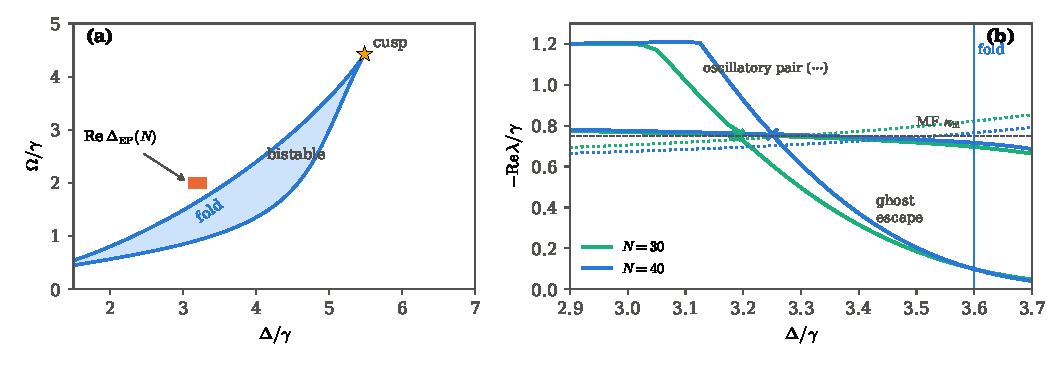
\includegraphics[width=\textwidth]{../figs/rev_fig1.pdf}
\caption{(a) MF bistable wedge (shaded) bounded by fold lines (blue) and terminating at a cusp (star). At $\Omega=2$, ticks mark ${\rm Re}\,\Delta_{\rm EP}(N)$ for $N=20$--$58$; they drift toward the left fold from outside the wedge. (b) Slowest real modes of the exact $\Lc_N$ near the left fold ($N=30,40$; solid). The ghost-escape branch (falling toward the fold) undergoes an avoided crossing with the high-branch relaxation mode, which stays near the MF value $\kappa_{\rm hi}$ (dashed). Crosses: real parts of the exact complex-$\Delta$ EP eigenvalue and location. Dotted: the oscillatory pair, which is slower than both real modes in part of this window.}
\label{fig:spec}
\end{figure*}

\emph{Model and MF geometry.}---We consider $N$ two-level atoms with uniform interaction $V/N$ and local decay $\hat L_i=\sqrt\gamma\,\hat\sigma^-_i$:
\begin{equation}
\hat H=-\Delta\hat N_e+\Omega\hat J_x+\tfrac{V}{2N}\hat N_e(\hat N_e-1).
\label{eq:H}
\end{equation}
We set $\gamma=1$ and $V=10$. Permutation symmetry reduces $\Lc_N$ to dimension $\binom{N+3}{3}$~\cite{Shammah2018}, which allows sparse shift-invert diagonalization up to $N=70$. In the limit $N\to\infty$, Eq.~\eqref{eq:H} gives Bloch equations with detuning $\Delta-Vn$, where $n=\langle\hat N_e\rangle/N$. The stationary populations solve a cubic, which has three roots inside the wedge of Fig.~\ref{fig:spec}(a). At a fold two roots merge. Eliminating the coherences, the characteristic polynomial of the Bloch Jacobian on the fold reduces exactly to
\begin{equation}
\chi(\lambda)=\lambda\big[(\lambda+1)^2+\Omega^2/2\big].
\label{eq:jac}
\end{equation}
The zero eigenvalue is simple even at the cusp, so no Jordan block appears in the Jacobian. The ``third-order'' structure lives only in the fixed-point equation (a triple root). At the fold, the surviving high branch relaxes with real rate $\kappa_{\rm hi}=0.751$ ($\Omega=2$).

\emph{The avoided crossing near the fold.}---Figure~\ref{fig:spec}(b) shows the real part of the slow spectrum of $\Lc_N$ across the left fold. The zero mode is always simple. Two real branches undergo an avoided crossing whose gap closes rapidly with $N$. We locate the EP at complex detuning $\Delta_{\rm EP}(N)$ by Newton iteration on the discriminant of the two eigenvalues. The residual is below $10^{-12}$, and the eigenvector overlap is $1-2\times10^{-14}$ at $N=30$. Encircling $\Delta_{\rm EP}$ in the complex plane exchanges the two branches, the hallmark of a square-root branch point. Because $\Lc$ is linear in $\Delta$, this EP is the analytic continuation of the avoided crossing; any real-axis avoided crossing has such a complex-$\Delta$ partner, at which $\Lc$ no longer preserves Hermiticity. The EP is therefore not a physical degeneracy, and what is specific to the fold is which modes cross and what sets their gap. The two-level relation ${\rm Im}\,\Delta_{\rm EP}=2g_N/|s_a-s_b|$, with $g_N$ the half-gap and $s_{a,b}$ the diabatic slopes, holds to $0.2\%$ at $N=40$. Two facts are therefore physical: the coupling $g_N$ on the real axis, and the drift of the crossing toward the fold.

The colliding modes are identified by their excitation-number profiles [Fig.~\ref{fig:modes}(a)]. One mode lives in the high basin. At the crossing its rate tracks the MF relaxation rate of the high branch evaluated at the same detuning: the difference falls from $0.038$ to $0.014$ between $N=20$ and $56$. Because the crossing location drifts with $N$, ${\rm Re}\,\lambda_{\rm EP}$ itself drifts slowly, from $-0.749$ to $-0.760$. Extrapolations with $N^{-p}$ corrections ($p=1/3$--$1$) give $-0.767$ to $-0.787$, i.e.\ a finite rate somewhat larger than the value $\kappa_{\rm hi}=0.751$ at the fold. The other mode has an $O(1)$ population peak at $n\simeq0.15$, close to the fold population $n_f=0.157$. It is the escape mode of the ghost left behind by the vanished low branch. The crossing therefore does not involve the MF zero mode. This explains why $\lambda_{\rm EP}$ stays finite while the crossing location drifts toward the fold. Figure~\ref{fig:modes}(b) shows the two scales: ${\rm Re}\,\Delta_{\rm EP}$ drifts toward the fold algebraically, roughly as $N^{-0.54}$, and ${\rm Im}\,\Delta_{\rm EP}$ decays exponentially, with local exponent $0.157$. The half-gap $g_N$ decays with a different exponent, $\sigma\simeq0.141$; the difference from ${\rm Im}\,\Delta_{\rm EP}$ comes from the $N$-dependent diabatic slopes. Below, $\sigma$ always refers to $g_N$. A parameter-free fold normal form, combined with the condition that the ghost-escape rate equal $\kappa_{\rm hi}$, accounts for $64$--$80\%$ of the real drift over $N=20$--$58$, and the agreement improves with $N$. This places the crossing in the right region. The central question is the origin of the exponent $\sigma$.

\begin{figure}[t]
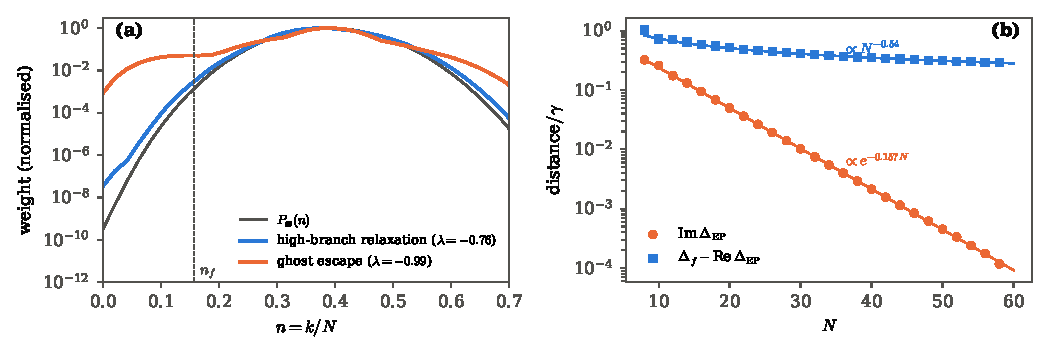
\includegraphics[width=\columnwidth]{../figs/rev_fig2.pdf}
\caption{(a) Excitation-number profiles of the two modes adjacent to the crossing ($N=48$, $\Omega=2$), with the steady-state distribution. The high-branch mode reaches the ghost region $n\approx n_f$ only through an exponentially small tail. (b) EP location: distance of ${\rm Re}\,\Delta_{\rm EP}$ from the fold (algebraic) and ${\rm Im}\,\Delta_{\rm EP}$ (exponential); lines are fits.}
\label{fig:modes}
\end{figure}

\emph{Instanton theory of the quasipotential.}---To predict $\Phi$ without input from the exact steady state, we use the real-time instanton approach of Refs.~\cite{PCE2026L,CEP2026}. Those works build it on Husimi/P quasiprobabilities; we use an equivalent coherent-state (Doi) form adapted to the permutation-symmetric Liouville space. In this space $\Lc_N$ describes $N$ bosons in four single-atom Liouville modes, and the large-$N$ action is generated by
\begin{equation}
h={\rm Re}\,{\rm Tr}\big[\hat X\,\ell_0(\hat\rho)\big]+2V\,{\rm Re}A\,{\rm Im}A,\qquad A={\rm Tr}(\hat X\hat n\hat\rho),
\label{eq:h}
\end{equation}
where $\hat\rho$ is a single-atom density matrix, $\hat X$ its conjugate, and $\ell_0$ the single-atom Lindbladian [Supplemental Material (SM)]. Gauge fixing ${\rm Tr}(\hat X\hat\rho)=1$ leaves three canonical pairs. We obtain heteroclinics by Lin's method, matching shots from the unstable manifold of the high fixed point and from the target manifold on a section. As a check, the switching action reproduces the exact exponent $s_{\rm hl}$ of the slowest eigenvalue to within $0.1$--$2.8\%$ [Fig.~\ref{fig:wkb}(a)]. In line with Refs.~\cite{PCE2026L,CEP2026}, a Gaussian-noise reduction overestimates it ($15$--$23\%$); an incoherent rate-equation reduction underestimates it by a factor of five.

The ingredient specific to the quasipotential of a \emph{measured} quantity is its endpoint. The excitation-number distribution $P(k)$ is the Fock coefficient of the Liouville bosons at occupation $x=\hat X\!\circ\!\hat\rho=(1-n,n,0,0)$, with $n=k/N$. Its rate function is therefore the Cole--Hopf action to that occupation point,
\begin{equation}
\Phi(n)=\int p\,dq+(1-n)\ln\hat X_{gg}+n\ln\hat X_{ee}.
\label{eq:phi}
\end{equation}
On the relevant endpoint branch ($p_u=p_v=0$) the boundary term equals $D(n\|n_{\hat\rho})$, the Kullback--Leibler cost of projective counting. Computed a priori, Eq.~\eqref{eq:phi} matches the $N\to\infty$ extrapolation of $-N^{-1}\ln P(k)$ to within $0.2$--$6\%$ [Fig.~\ref{fig:wkb}(b); pre-registered].

\begin{figure}[t]
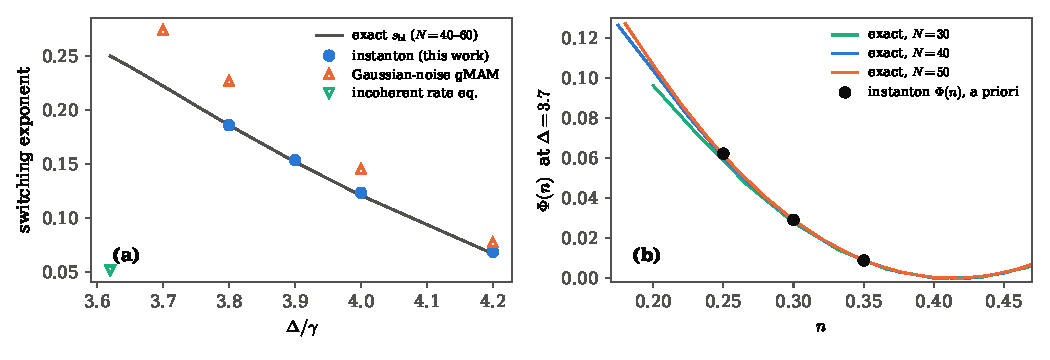
\includegraphics[width=\columnwidth]{../figs/rev_fig3.pdf}
\caption{Instanton inputs at $\Omega=2$. (a) Switching exponent: exact (line), instanton (dots), Gaussian-noise minimum action (open triangles), incoherent rate equation (open). (b) Quasipotential of the excitation number at $\Delta=3.7$: exact finite-$N$ curves and the a-priori instanton values from Eq.~\eqref{eq:phi}.}
\label{fig:wkb}
\end{figure}

\emph{Prediction of the EP coupling.}---Figure~\ref{fig:modes}(a) suggests a simple mechanism. The ghost mode is $O(1)$ at $n_f$, whereas the high-branch mode reaches $n_f$ only through its exponentially small large-deviation tail. Their overlap is the coupling, so
\begin{equation}
g_N\simeq c\,\exp\!\big[-N\,\Phi(n_f;\Delta_{\min}(N))\big],
\label{eq:pred}
\end{equation}
where $\Delta_{\min}(N)$ is the crossing location. Equation~\eqref{eq:pred} is a heuristic: for a non-Hermitian two-mode reduction the half-gap is $\sqrt{V_{ab}V_{ba}}$, and we have not shown that the product of the two cross elements scales as $e^{-2N\Phi(n_f)}$. We tested Eq.~\eqref{eq:pred} in two pre-registered steps, on parameters not used to formulate it, with exact couplings sealed until the predictions were frozen. (v3) With $\Phi$ read from the exact steady state at $\Omega=2.5$ and $3.0$, the fitted slopes of $\ln g_N$ vs $N\Phi$ are $0.957$ and $0.878$; the local exponents are $0.944$ and $0.878$ of the predicted values. (v4) With $\Phi$ from Eq.~\eqref{eq:phi} computed a priori and $\Delta_{\min}$ as the only spectral input, at $\Omega=2.25$ and $2.75$: slopes $0.958$ and $0.929$, local-exponent ratios $0.963$ and $0.934$ [Fig.~\ref{fig:pred}]. All registered criteria ($1\pm0.15$) passed.

These tests are weaker than they appear. Over $\Omega\in[2.25,3]$, $\Phi(n_f)$ changes by only $\sim10\%$. A null model with no physics, which carries the exponent $\sigma=0.141$ measured at the formation point $\Omega=2$ forward to all $\Omega$, passes three of the four criteria (ratios $1.02,1.0,0.94,0.84$). The relation does track the $\Omega$ dependence: the observed $\sigma$ (from $0.142$ to $0.118$) and the predicted values are correlated with coefficient $0.998$, and after removal of a common offset the residuals are $0.004$, versus $0.010$ for the constant null. However, the predictions overshoot systematically by $4$--$12\%$ (largest at $\Omega=3$), and this offset is not explained. It is not a finite-$N$ prefactor effect in $\Phi$: the v3 tests use the exact finite-$N$ $\Phi_N$ and overshoot as much or more. The evaluation point is pinned only to $n_f\pm0.02$; nearby points such as the ghost-mode peak are not excluded. Two earlier candidates were tested at the formation point $\Omega=2$ and failed by factors of $2$--$4$: the action to the MF fold \emph{state} (not formally pre-registered), and the action to a bottleneck hyperplane imposed in $\hat\rho$ coordinates (pre-registered; its solver was corrected once during the run). Both suggest that the endpoint must be imposed on occupations rather than on density matrices.

\begin{figure}[t]
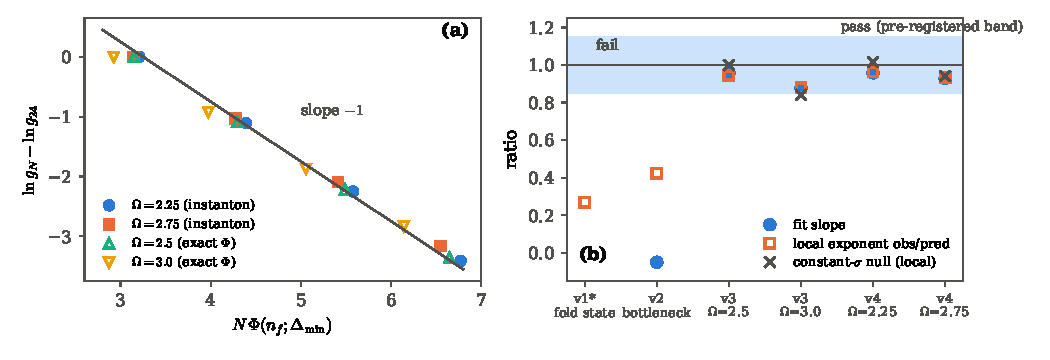
\includegraphics[width=\columnwidth]{../figs/rev_fig4.pdf}
\caption{(a) Coupling of the avoided crossing vs $N\Phi(n_f)$ at four drive strengths not used to construct Eq.~\eqref{eq:pred}. Filled: $\Phi$ from the a-priori instanton calculation. Open: $\Phi$ from the exact steady state. The line has slope $-1$. (b) Tests of Eq.~\eqref{eq:pred}. v1 (not formally registered) and v2 used other endpoint definitions at $\Omega=2$ and failed. v3 and v4 fall inside the registered band; so does a constant-exponent null in three of four cases (see text).}
\label{fig:pred}
\end{figure}

\emph{Discussion.}---The many-body counterpart of the MF ``exceptional line'' is an avoided crossing of two decaying modes of distinct physical origin; it is not a coalescence of steady states. Our data are consistent with its gap being set by the large-deviation cost of populating the ghost region from the surviving branch, $\sigma\simeq\Phi(n_f)$. A sharp test requires parameters where $\Phi(n_f)$ varies strongly, near the cusp where $\Phi(n_f)\to0$, at other $V$, and at the opposite fold, together with a derivation from a biorthogonal two-mode reduction. Compared with the driven-oscillator EP of Ref.~\cite{Cabot2024}, which separates phase diffusion from activation, the present EP accompanies a saddle-node and couples a relaxation mode to an escape mode. If confirmed, the relation would depend only on the structure of the fold, an $O(1)$ ghost mode at $n_f$ and a large-deviation tail of the intrabasin mode reaching it, and should then hold in other permutation-symmetric bistable systems.

For many-body chiral switching~\cite{Xie2025}, two further results follow (SM). In the quasi-static MF limit, the final branch is fixed by the fold through which the bistable arc is last entered; encircling the cusp is not required. This holds in the published MF models of Ref.~\cite{Xie2025}, where a loop that does not enclose the cusp switches. In the exact dynamics, direction memory decays as $\exp(-T\Lambda_N)$, where $\Lambda_N$ is the switching rate integrated from the Maxwell point.

\emph{Scope.}---All statements refer to the permutation-symmetric model of Eq.~\eqref{eq:H}. Short-range interactions can replace collective switching by nucleation~\cite{Xiang2026}, and we have not addressed that case. The algebraic drift of ${\rm Re}\,\Delta_{\rm EP}$ is not yet asymptotic for $N\le58$, so convergence of the crossing to the fold remains a conjecture and we do not quote a limiting exponent. The crossing location $\Delta_{\min}(N)$ still enters Eq.~\eqref{eq:pred} as an exact spectral input. Pre-registration documents and all code and data are provided as SM.

\begin{thebibliography}{99}
\bibitem{Carr2013} C.~Carr, R.~Ritter, C.~G.~Wade, C.~S.~Adams, and K.~J.~Weatherill, Phys. Rev. Lett. \textbf{111}, 113901 (2013).
\bibitem{Xie2025} C.~Xie, K.~Sun, K.-D.~Wu, C.-F.~Li, G.-C.~Guo, W.~Yi, and G.-Y.~Xiang, Sci. Bull. \textbf{70}, 3345 (2025); arXiv:2402.02779.
\bibitem{Casteels2017} W.~Casteels, R.~Fazio, and C.~Ciuti, Phys. Rev. A \textbf{95}, 012128 (2017).
\bibitem{Minganti2018} F.~Minganti, A.~Biella, N.~Bartolo, and C.~Ciuti, Phys. Rev. A \textbf{98}, 042118 (2018).
\bibitem{Macieszczak2016} K.~Macieszczak, M.~Gu\c{t}\u{a}, I.~Lesanovsky, and J.~P.~Garrahan, Phys. Rev. Lett. \textbf{116}, 240404 (2016).
\bibitem{SunYi2024} K.~Sun and W.~Yi, AAPPS Bull. \textbf{34}, 22 (2024).
\bibitem{HuBudich2025} Y.-M.~Hu and J.~C.~Budich, Phys. Rev. Lett. \textbf{135}, 250402 (2025).
\bibitem{Ptaszynski2024} K.~Ptaszy\'nski and M.~Esposito, arXiv:2407.07832.
\bibitem{Xiang2026} Y.-X.~Xiang, W.~Li, Z.~Bai, and Y.-Q.~Ma, Natl. Sci. Rev. \textbf{13}, nwag146 (2026).
\bibitem{Krimer2019} D.~O.~Krimer and M.~Pletyukhov, Phys. Rev. Lett. \textbf{123}, 110604 (2019).
\bibitem{PCE2026L} K.~Ptaszy\'nski, M.~Chudak, and M.~Esposito, arXiv:2604.15091.
\bibitem{CEP2026} M.~Chudak, M.~Esposito, and K.~Ptaszy\'nski, arXiv:2610.21684.
\bibitem{Cabot2024} A.~Cabot, G.~L.~Giorgi, and R.~Zambrini, PRX Quantum \textbf{5}, 030325 (2024).
\bibitem{Shammah2018} N.~Shammah, S.~Ahmed, N.~Lambert, S.~De~Liberato, and F.~Nori, Phys. Rev. A \textbf{98}, 063815 (2018).
\end{thebibliography}

\end{document}
